\documentclass[../../main.tex]{subfiles}

\begin{document}

\paragraph{Sagsåbning GUI Mockup}\mbox{} \\
Gruppens udkast for “Sagsåbning GUI Mockup” tager udgangspunkt i det detaljeret \\ 
brugsmønstre for sagsåbning. Udkastet havde til fokus at vise hvordan brugeren skulle bruge funktionalitet i systemet. Derudover skulle “Sagsåbning GUI Mockup” være en grundtegning for udviklerne der skulle designe brugergrænsefladen for sagsåbningen. “Sagsåbning GUI Mockup” er dog stadige et udkast for selve brugergrænsefladen som kun har fokus på funktionalitet, og har derfor ikke taget højde for brugervenlighed. Fokus på brugervenlighed vil der bliver sat fokus på længer inde i udviklingen af brugergrænsefladen. “Sagsåbning GUI Mockup” består af et log-in window, oversigts window og et vindue for være enkel brugsmønstre i sagsåbningen.


\begin{center}
\begin{figure}[H]
  \centering
  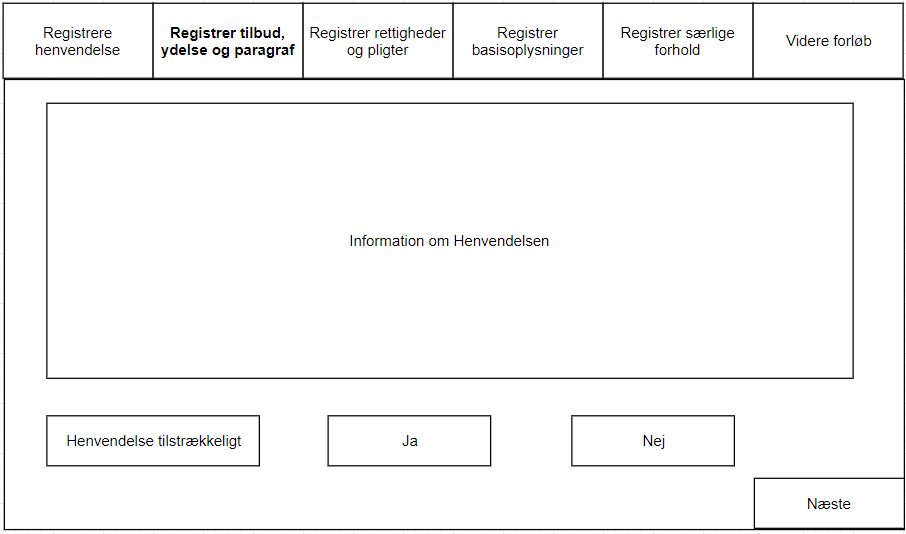
\includegraphics[scale=.5]{figurer/Sags_bning_GUI_Mockup.PNG}
  \caption{GUI Mockup af Sagsåbning}
  \label{fig:forhold_sekvensdiagram}
\end{figure}
\end{center}


\end{document}
